\documentclass{article}
\usepackage[T1]{fontenc}
\usepackage[utf8]{inputenc}
\usepackage{amsmath, amssymb, amsthm}
\usepackage{graphicx}
\usepackage{bigints}
\usepackage{tikz}

\title{Complex Analysis}
\author{B Ritukanta Reddy}

\begin{document}

\maketitle

\section{Complex Numbers and Properties}
\subsection{Definitions}

A complex number is a number of the form $z=x + iy$, where $x$, $y$ are real numbers and $i$ is the imaginary unit, satisfying the equation $i^2 = -1$. The set of complex numbers is denoted by $\mathbb{C}$.
\\
\[
\boxed{\mathbb{C} = \{x+iy \mid x,y \in \mathbb{R}, i=\sqrt{-1}\}}
\]
\begin{itemize}
    \item For any complex number $z=x+iy$, $x$ is called the real part of $z$ and $y$ is called the imaginary part of $z$. That is, $Re(z)=x$ and $Im(z)=y$.
    \item Since $i=\sqrt{-1}$, we have
    \[
    \Rightarrow i^2=-1
    \]
    \[
    \Rightarrow i^4=1
    \]
    Hence $i^{4m}=1$ for any $m\in \mathbb{Z}$.
    \item The conjugate of a complex number $z=x+iy$ is given by $\overline{z}=x-iy$. 
    \item Modulus of a complex number $z$, $|z|=\sqrt{x^2+y^2}$
\end{itemize}

\subsection{Properties}
If $z_1=a+ib$ and $z_2=c+id$ where $z_2 \neq 0$, then
\begin{itemize}
    \item $z_1+z_2=(a+c)+i(b+d)$
    \item $z_1-z_2=(a-c)+i(b-d)$
    \item $z_1 z_2=(ac-bd)+i(ad+bc)$
    \item $\frac{z_1}{z_2}=(\frac{ac+bd}{c^2+d^2})+i (\frac{bc-ad}{c^2+d^2})$
    \item $arg(z_1)= \theta=tan^{-1} \frac{b}{a}$
    \item Polar form of a complex number $z=x+iy$ having $|z|=r$ is given by 
    \[
    z=r\cos\theta+ir\sin\theta
    \]
    \[
    \Rightarrow z=r(\cos\theta+i\sin\theta)
    \]
    \[
    \Rightarrow z=re^{i\theta}
    \]
    \item $arg(z_1 z_2)=arg(z_1)+arg(z_2)$
    \item $arg \frac{z_1}{z_2}=arg(z_1)-arg(z_2)$
    \item $arg(z^n)=n*arg(z)$
    \item $|z|^2=z\overline{z}$%
\end{itemize}
\subsection{Examples}
\begin{itemize}
    \item Evaluate $\displaystyle \int_{0}^{2\pi}\cos^4\theta d\theta$.
    \\
    \\
    \underline{Solution.} We have that, 
    \[
    \cos\theta= \frac{e^{i\theta}+e^{-i\theta}}{2}
    \]
    \[
    \Rightarrow cos^4\theta= \Big(\frac{e^{i\theta}+e^{-i\theta}}{2}\Big)^4
    \]
    \[
    =\frac{1}{16}(e^{4i\theta}+4e^{3i\theta}.e^{-i\theta}+6e^{2i\theta}.e^{-2i\theta}+4e^{i\theta}.e^{-3i\theta}+e^{-4i\theta})
    \]
    \[
    =\frac{1}{16}(e^{4i\theta}+4e^{2i\theta}+6e^0+4e^{-2i\theta}+e^{-4i\theta})
    \]
    \[
    =\frac{1}{16}[(e^{4i\theta}+e^{-4i\theta})+4(e^{2i\theta}+e^{-2i\theta})+6]
    \]
    \[
    = \frac{1}{16}(2\cos4\theta+8\cos2\theta+6)
    \]
    \[
    =\frac{1}{8}(\cos4\theta+4\cos2\theta+3) 
    \]
    \begin{align}
        \therefore \displaystyle \int_{0}^{2\pi}\cos^4\theta d\theta &= \displaystyle\int_{0}^{2\pi}\frac{1}{8}(\cos^4\theta+4\cos2\theta+3)d\theta \\
        &= \frac{1}{8}(\frac{1}{4}\sin4\theta+\frac{4}{2}\sin2\theta+3\theta) \bigg|_{0}^{2\pi}\\
        &=\frac{1}{8}(\frac{1}{4}\sin8\pi+2\sin4\pi+6\pi\ -\frac{1}{4}\sin0-2\sin0-0)\\
        &=\frac{1}{8}.6\pi\\
        &=\frac{3\pi}{4} \qed
    \end{align}
\end{itemize}
\section{Sequences of Complex Numbers}
\subsection{Convergence}
A sequence $\{z_n\}$ of complex numbers is said to converge to a complex number $w$ if for every $\epsilon >0$ there exists a positive integer $n_0$ such that $|z_n-w|<\epsilon$ for all $n_\geq n_0$. \textbf{OR} a sequence of complex numbers is said to converge to $w\in \mathbb{C}$ if 
\[
\boxed{\lim_{n \to \infty}z_n=w}
\].
\subsection{Cauchy Sequence}
A sequence $\{z_n\}$ of complex numbers is said to be Cauchy if for every $\epsilon >0$ there exists $n_0 \in \mathbb{N}$ such that  $|z_n-z_m|<\epsilon$ for all $m,n\geq n_0$.

For any $z_n=x_n+iy_n$, $\{z_n\}$ is Cauchy if and only if $\{x_n\}$ and $\{y_n\}$ are Cauchy.
\subsection{Theorem: $\mathbb{C}$ is complete}
\underline{Statement} $\mathbb{C}$, the set of complex numbers, is complete.
\\
\\

\underline{Proof} Let $z_n=x_n+y_n$ form a Cauchy sequence then $\{x_n\}$ and $\{y_n\}$ are Cauchy. Since $\mathbb{R}$ is complete, $\{x_n\}$ and $\{y_n\}$ converge to $x$ and $y$ in $\mathbb{R}$ respectively. Then for any $\epsilon>0$ there exist two natural numbers $n_1$ and $n_2$ such that $|x_n-x|<\frac{\epsilon}{2}$ and $|y_n-y|<\frac{\epsilon}{2}$.
\\
\\
Now choose $n_0=max\{n_1, n_2\}$ and let $w=x+iy$.
\\
 \begin{align}
     \therefore |z_n-w|&= |(x_n+iy_n)-(x+iy)| \\
     &=|(x_n-x)+i(y_n-y)|\\
     &\leq|x_n-x|+|y_n-y|\\
     &<\frac{\epsilon}{2}+\frac{\epsilon}{2}\\
     &<\epsilon
 \end{align}
\\
So for any $\epsilon>0$ there exists $n \in \mathbb{N}$ such that $|z_n-w|<\epsilon$ for all $n \geq n_0$
\\
Thus $\{z_n\}$ converges to $w$, hence $\mathbb{C}$ is complete.\qed
\\
\section{Sets in Complex Plane}
\subsection{Open Disc}
$D_r(z_0)=\{z\in \mathbb{C} \mid |z-z_0|<r\}$
\subsection{Closed Disc}
$\overline{D_r}(z_0)=\{z\in \mathbb{C} \mid |z-z_0| \leq r\} $
\subsection{Interior Point}
Given a set $\Omega \subset \mathbb{C}$, a point $z_0$ is an interior point of $\Omega$ if there exists $r>0$ such that
\\
$D_r(z_0)=\{z\in \mathbb{C} \mid |z-z_0|<r\} \subset \Omega$.
\subsection{Open Set}
A set $\Omega \subset \mathbb{C}$ is open if every point in $\Omega$ is an interior point of $\Omega$.
\subsection{Interior}
The interior of $\Omega$ consists of all its interior points.
\subsection{Limit Point}
A point $z \in \mathbb{C}$ is said to be a limit point of a set $\Omega \subset \mathbb{C}$ if there exists a sequence points $z_n \in \Omega$ s.t. $z_n \neq z$ and 
\[
\lim_{n \to \infty} z_n=z
\]
\subsection{Closed Set}
A set $\Omega \subset \mathbb{C}$ is closed if $\Omega^c=\mathbb{C}-\Omega$ is open.
\subsection{Closure($\overline{\Omega}$)}
The closure of any set $\Omega$ is the union of $\Omega$ and its limit points.
\subsection{Diameter}
If $\Omega$ is bounded, we define its diameter by
\\
\[
diam(\Omega)=Sup_{z,w \in \Omega}|z-w|
\]
\subsection{Compact Set}
A set $\Omega$ is said to be compact if it is closed and bounded.
\subsection{Open Covering}
An open covering of a set $\Omega$ is the family of open sets $\{U_\alpha\}$ (not necessarily countable) such that $\Omega \subset \{U_\alpha\}$.
\subsection{Connected Sets}
An open set $\Omega \subset \mathbb{C}$ is said to be connected if it is not possible to find two disjoint non-empty open sets $\Omega_1$ and $\Omega_2$ s.t.
$\Omega=\Omega_1\cup \Omega_2$.
\section{Complex-valued Functions}
Let $\Omega \subset \mathbb{C}$, a function is defined on $\Omega$ is a rule which assigns every $z \in \Omega$ to a complex number $w$ i.e. $f(z)=w$.
\begin{itemize}
    \item For $w=f(z)=u(z)+iv(z)$, $Re(f)=u$ and $Im(f)=v$.
\end{itemize}
\subsection{Examples}
\begin{itemize}
    \item Given $f(z)=\frac{z}{1+z}$, find real and imaginary part of $f$..
    \\
    \\
    \underline{Solution.} Let $z=x+iy$, for $x,y \in \mathbb{R}$
    \\
    \begin{align}
        f(z) &= \frac{x+iy}{1+(x+iy)} \\
        &=\frac{x+iy}{(1+x)+iy} \\
        &=\frac{x+iy}{(1+x)+iy}* \frac{(1+x)-iy}{(1+x)-iy} \\
        &=\frac{x+x^2-ixy+iy+ixy-i^2y^2}{(1+x)^2-i^2y^2} \\
        &=\frac{x+x^2+y^2+iy}{(1+x)^2+y^2} \\
        &=\frac{x^2+y^2+x}{(1+x)^2+y^2}+i \frac{y}{(1+x)^2+y^2}
    \end{align}
    \\
    \\
    $Re(f)=\frac{x^2+y^2+x}{(1+x)^2+y^2}$ and $Im(f)=\frac{y}{(1+x)^2+y^2}$
    
    
    \item Find the domain of $f(z)=\frac{1}{z^2+4}$.
    \\
    \\
    \underline{Solution.} $f(z)$ is not defined for $z^2+4=0$
\[     \Rightarrow z^2=-4     \] \[     \Rightarrow z=\sqrt{-4}     \] \[     \Rightarrow z=\pm 2i     \] Therefore, the domain of $f$ is $\mathbb{C}-\{\pm2i\}$.
\end{itemize}
\subsection{Region}
A non-empty open connected subset of $\mathbb{C}$ is called a region.
\subsection{Domain}
An open connected set is called a domain.
\subsection{Limit of a Function}
Consider a function $f(z)$ defined on $D$, we say that $L$ is the limit of the function $f(z)$ as $z \to z_0$ if for every $\epsilon>0$ there exists $\delta>0$ s.t.
\\
\\
$|f(z)-L|<\epsilon$ whenever $|z-z_0|<\delta$.
\begin{itemize}
    \item We say that $\lim_{z \to z_0}f(z)=L$.
\end{itemize}
\subsection{Algebra of Limits}
Let $f$ and $g$ be two complex valued functions defined in a neighbourhood of $z_0$ except possibly at $z_0$ and given that $\lim_{z \to z_0}f(z)=L$ and $\lim_{z \to z_0}g(z)=M$, then
\begin{itemize}
    \item $\lim_{z \to z_0}[f(z) \pm g(z)]=L\pm M$
    \item $\lim_{z \to z_0}f(g(z))=LM$
    \item $\lim_{z\to z_0}\frac{f}{g}(z)=\frac{L}{M}$ for $M\neq 0$.
    \item $\lim_{z\to z_0}\overline{f(z)}=\overline{L}$
    \item $\lim_{z\to z_0}|f(z)|=|L|$.
\end{itemize}
\subsection{Limit at Infinity}
\[
\lim_{z\to \infty}f(z)=L
\]
if for given $\epsilon>0$ there exists any $R>0$ s.t.
\\
\\
$|f(z)-L|<\epsilon$ for $|z|>R$.
\subsection{Infinite Limits}
$\lim_{z\to z_0}f(z)=\infty$ if for given $R>0$ there exists $\delta>0$ s.t.
\\
\\
$|f(z)>R$ if $|z-z_0|<\delta$.
\subsection{Continuous Functions}
Let $f$ be complex valued function defined on a set $\Omega$ of complex numbers. We say $f$ is continuous at a point $z_0\in \Omega$ if for every $\epsilon>0$ there exists $\delta>0$ such that
\\
\\
$|f(z)-f(z_0)|<\epsilon$ whenever $|z-z_0|<\delta$.
\\
\\
If $f$ is continuous at $z_0$, then:
\begin{itemize}
    \item $Re(f)$ is continuous at $z_0$
    \item $Im(f)$ is continuous at $z_0$
    \item $\overline{f}$ is continuous at $z_0$
    \item $|f|$ is continuous at $z_0$
    \item $\alpha f$ is continuous at $z_0$, where $\alpha$ is any scalar.
\end{itemize}
\section{Differentiability, Holomorphic Functions or Analytic Functions}
\subsection{Definition}
Let $f$ be a complex-valued function in a domain $\Omega$ then $f$ is said to be holomorphic at a point $z_0\in \Omega$ if the limit:
\\
\\
\[
\boxed{\lim_{h \to 0}\frac{f(z_0+h)-f(z_0)}{h}}
\]
exists and we denote it as $f'(z_0)$.
\begin{itemize}
    \item If $f$ is holomorphic at every point of $\Omega$ then $f$ is called holomorphic on $\Omega$.
    \item If $\Omega$ is a closed subset of $\mathbb{C}$ then we say that $f$ is holomorphic on $\Omega$ if $f$ is holomorphic on an open set containing $\Omega$.
\end{itemize}
\subsection{Entire Functions}
A function $f$ is said to be entire if $f$ is holomorphic entirely on $\mathbb{C}$.
\subsection{Analytic Functions}
A function $f(z)=u(x,y)+iv(x,y)$ is analytic if
\begin{itemize}
    \item $f$ satisfies Cauchy-Riemann equations:
    \begin{align}
        u_x&=v_y \\
        u_y&=-v_x
    \end{align}
    \item $u_x$, $u_y$, $v_x$ and $v_y$ exist and are continuous.
\end{itemize}
\subsection{Theorem}
Suppose $f(z)=u(x,y)+iv(x,y)$ is complex valued function on an open set $\Omega$. If $u$ and $v$ are continuously differentiable and satisfy $C-R$ equations on $\Omega$, then $f$ is holomorphic on $\Omega$ and $f'(z)=\frac{\partial f}{\partial z}$.
\\
\\
\underline{Proof :-} Given that $(i)$ $u$ and $v$ are continuously differentiable and $(ii)$ both satisfy $C-R$ equations on $\Omega$.
\begin{center}
    To show that $f$ is holomorphic, we have to prove that $f$ is complex differentiable at every point of $\Omega$. $f$ is differentiable at a point $z\in \Omega$ if the limit:

\end{center}

\[
f'(z)=\lim_{h\to 0}\frac{f(z+h)-f(z)}{h}
\]
exists, where $h$ is a complex constant.
\\
\\
Let $z=x+iy$ and $h=\Delta x+i\Delta y$.
\\
So, $f(z)=u(x,y)+iv(x,y)$
\\
and \begin{align}
    f(z+h)&=f((x+iy)+(\Delta x+i\Delta y)) \\
    &=f((x+\Delta x)+i(y+\Delta y)) \\
    &=u(x+\Delta x, y+\Delta y)+iv(x+\Delta x, y+\Delta y)
\end{align}
\\
\\
Now, \begin{align}
    \frac{f(z+h)-f(z)}{h} &= \frac{[u(x+\Delta x,y+\Delta y)+iv(x+\Delta x,y+\Delta y)]-[u(x,y)+iv(x,y)]}{\Delta x+i\Delta y} \\
    &=\frac{[u(x+\Delta x,y+\Delta y)-u(x,y)]+i[v(x+\Delta x,y+\Delta y)-v(x,y)]}{\Delta x+i\Delta y}
\end{align}
\\
\\
Using Taylor's series expansion of a function $g(x,y)$,
\\
\\
$g(x+\Delta x,y+\Delta y)-g(x,y)=g_x\Delta x+g_y\Delta y+O(|h|)$
\\
\\ where $O(|h|) \to 0$ faster than $|h|$ when $h\to 0$. That is,
\\
\\

\[
\boxed{\lim_{h\to 0}\frac{O(|h|)}{h}=0}
\]
\\
\\
Equation $(13)$ becomes,
\\
\\
\begin{align}
    \frac{f(z+h)-f(z)}{h}&=\frac{[u_x\Delta x+u_y\Delta y+O(|h|)]+i[v_x\Delta x+v_y\Delta y+O(|h|)]}{\Delta x+i\Delta y}
\end{align}
By $C-R$ equations, $u_x=v_y$ and $u_y=-v_x$,
So
\\
\\
\begin{align}
    \frac{f(z+h)-f(z)}{h}&=\frac{[u_x\Delta x-v_x\Delta y+O(|h|)]+i[v_x\Delta x+u_x\Delta y+O(|h|)]}{\Delta x+i\Delta y} \\
    &=\frac{\Delta x(u_x+iv_x)+\Delta y(iu_x-v_x)+O(|h|)(1+i)}{\Delta x+i\Delta y}\\
    &=\frac{\Delta x(u_x+iv_x)+i\Delta y(u_x+iv_x)}{\Delta x+i\Delta y}+\frac{O(|h|)(1+i)}{h}\\
    &=\frac{(\Delta x+i\Delta y)(u_x+iv_x)}{\Delta x+i\Delta y}+\frac{O(|h|)(1+i)}{h}\\
    &=(u_x+iv_x)+\frac{O(|h|)(1+i)}{h}
\end{align}
Taking $\lim_{h\to 0}$ both sides,
\begin{align}
    f'(z)&=\lim_{h\to 0}\frac{f(z+h)-f(z)}{h} \\
    &= \lim_{h\to 0}[(u_x+iv_x)+\frac{O(|h|)(1+i)}{h}] \\
    &=u_x+iv_x
\end{align}
\\
\\
This shows that $f$ is complex differentiable at any point of $\Omega$, therefore $f$ is holomorphic on $\Omega$.\qed
\newpage
\subsection{Conjugate Harmonic Functions}
Let $f=u+iv$ be an analytic function then $v$ is harmonic conjugate of $u$ and $u$ is harmonic conjugate of $-v$.
\\
\\
\begin{itemize}
    \item If $f=u+iv$ is an analytic function and $u$ is harmonic conjugate  of $v$ as well as $v$ is harmonic conjugate of $u$, then $f$ is constant.
    \item If $u$ is a harmonic function then $f(z)=u_x-iu_y$ is analytic.
    \item If $u$ and $v$ are conjugate harmonic functions, then $uv$ is harmonic.
\end{itemize}
\subsection{Problems on Analytic Functions}
\begin{itemize}
    \item Is $f$ analytic, if $f(z)=(2x-3y)+i(3x+2y)$?
    \\
    \underline{Solution.} Here 
    \begin{align}
    u(x,y)&=2x-3y \\
    v(x,y)&=3x+2y    
    \end{align}
    $u_x=2$,$u_y=-3$,$v_x=3$ and $v_y=2$
    \\
    $u_x=v_y$ and $u_y=-v_x$
    \\
    \\
    So $f$ is analytic.
    \item If $f=u+iv$ is analytic and $u=v^2$ then prove that $f$ is constant.
    \\
    \underline{Solution.} Given $u=v^2$
    \\
    \\
    Differentiating w.r.t. $x$ partially,
    \\
    \\
    $\frac{\partial u}{\partial x}=2v\frac{\partial v}{\partial x}$
    \\
    \\
    Again differentiating w.r.t. $y$ partially,
    \\
    \\
    $\frac{\partial u}{\partial y}=2v\frac{\partial v}{\partial y}$
    \\
    \\
    From the above,
    \\
    \\
    \begin{align}
        2v&=\frac{u_x}{v_x}=\frac{u_y}{v_y} \\
        \Rightarrow \frac{u_x}{v_x}&=\frac{-v_x}{u_x} \\
        \Rightarrow u_x^2&=-v_x^2 \\
        \Rightarrow u_x^2&=-(-u_y^2) \\
        \Rightarrow u_x^2+u_y^2=0 \\
    \end{align}
    So $u$ is constant $\Rightarrow$ $f$ is constant. \qed
\end{itemize}
\begin{itemize}
    \item Compute the complex form of $C-R$ equations.
    \\
    \\
    \underline{Solution.} 
The Cauchy-Riemann equations, for a complex function \( f(z) = u(x,y) + i v(x,y) \) are:

\[
\frac{\partial u}{\partial x} = \frac{\partial v}{\partial y}, \quad \frac{\partial u}{\partial y} = -\frac{\partial v}{\partial x}
\]

In terms of complex derivatives, using the Wirtinger derivatives:

\[
\frac{\partial}{\partial z} = \frac{1}{2} \left( \frac{\partial}{\partial x} - i \frac{\partial}{\partial y} \right), \quad
\frac{\partial}{\partial \bar{z}} = \frac{1}{2} \left( \frac{\partial}{\partial x} + i \frac{\partial}{\partial y} \right)
\]

The Cauchy-Riemann equations are equivalent to the condition:

\[
\frac{\partial f}{\partial \bar{z}} = 0
\]

which ensures that \( f(z) \) is holomorphic.
\item Test whether the function $e^x(\cos y-i\sin y)$ is analytic.
\\
\\
\underline{Solution.} 
Let
\[
f(z) = e^x (\cos y - i \sin y)
\]
\[
f(z) = e^x e^{-i y} = e^{x - i y}
\]
\[
f(z) = e^x \cos y - i e^x \sin y
\]
Thus, we define:
\[
u(x, y) = e^x \cos y, \quad v(x, y) = -e^x \sin y
\]

Compute the Partial Derivatives:

\[
\frac{\partial u}{\partial x} = e^x \cos y, \quad \frac{\partial u}{\partial y} = -e^x \sin y
\]
\[
\frac{\partial v}{\partial x} = -e^x \sin y, \quad \frac{\partial v}{\partial y} = -e^x \cos y
\]

Check the Cauchy-Riemann Equations:

The Cauchy-Riemann equations are:
\[
\frac{\partial u}{\partial x} = \frac{\partial v}{\partial y}, \quad \frac{\partial u}{\partial y} = -\frac{\partial v}{\partial x}
\]

Substituting:
\[
e^x \cos y \neq -e^x \cos y
\]
\\
\\
\\
$\therefore$ Given function $f$ is not analytic.\qed
\end{itemize}
\newpage
\begin{itemize}
    \item Compute the polar form of $C-R$ equations.
    \\
    \\
    \underline{Solution.} Let
    \begin{align}
        z&= x+iy\\
        &=r\cos\theta+ir\sin\theta\\
        &=re^{i\theta}
    \end{align}
    \\
    So $f(z)=u(r,\theta)+iv(r,\theta)$
    \\
    \\
    Differentiating the above equation w.r.t. $r$, partially
    \\
    \\
    \[
    f'(re^{i\theta})\frac{\partial}{\partial r}(re^{i\theta})=\frac{\partial u}{\partial r}+i\frac{\partial v}{\partial r} 
    \]
    \[
    \Rightarrow e^{i\theta}f'(re^{i\theta})=\frac{\partial u}{\partial r}+i\frac{\partial v}{\partial r}
    \]
    Again differentiating $f$ w.r.t. $\theta$ partially,
    \\
    \\
    \[
    f'(re^{i\theta})\frac{\partial}{\partial\theta}(re^{i\theta})=\frac{\partial u}{\partial \theta}+i\frac{\partial v}{\partial \theta}
    \]
    \[
    \Rightarrow rie^{i\theta}f'(re^{i\theta})=\frac{\partial u}{\partial \theta}+i\frac{\partial v}{\partial \theta}
    \]
    \[
    \Rightarrow ir(\frac{\partial u}{\partial r}+i\frac{\partial v}{\partial r})=\frac{\partial u}{\partial \theta}+i\frac{\partial v}{\partial \theta}
    \]
    \[
    \Rightarrow ir\frac{\partial u}{\partial r}-r\frac{\partial v}{\partial r}=\frac{\partial u}{\partial \theta}+i\frac{\partial v}{\partial \theta}
    \]
    \[
    \therefore \boxed{u_\theta=-rv_r}
    \]
    \[
    \boxed{u_r=\frac{1}{r}v_\theta}
    \]
    \qed
    \item Prove that $u(x,y)$ and $u(x^2-y^2, 2xy)$ are simultaneously harmonic.
    \\
    \\
    \underline{Solution.} A function \( u(x, y) \) is harmonic if it satisfies Laplace’s equation:  

\[
\frac{\partial^2 u}{\partial x^2} + \frac{\partial^2 u}{\partial y^2} = 0.
\]

Let \( u(x, y) \) be harmonic, meaning

\[
\frac{\partial^2 u}{\partial x^2} + \frac{\partial^2 u}{\partial y^2} = 0.
\]

Define new coordinates:

\[
X = x^2 - y^2, \quad Y = 2xy.
\]

Compute partial derivatives:

\[
\frac{\partial X}{\partial x} = 2x, \quad \frac{\partial X}{\partial y} = -2y, \quad \frac{\partial Y}{\partial x} = 2y, \quad \frac{\partial Y}{\partial y} = 2x.
\]

Apply the chain rule:

\[
\frac{\partial u}{\partial x} = \frac{\partial u}{\partial X} \frac{\partial X}{\partial x} + \frac{\partial u}{\partial Y} \frac{\partial Y}{\partial x} = 2x \frac{\partial u}{\partial X} + 2y \frac{\partial u}{\partial Y}.
\]

\[
\frac{\partial u}{\partial y} = \frac{\partial u}{\partial X} \frac{\partial X}{\partial y} + \frac{\partial u}{\partial Y} \frac{\partial Y}{\partial y} = -2y \frac{\partial u}{\partial X} + 2x \frac{\partial u}{\partial Y}.
\]

Differentiate again:

\[
\frac{\partial^2 u}{\partial x^2} = 2 \frac{\partial u}{\partial X} + 4x^2 \frac{\partial^2 u}{\partial X^2} + 8xy \frac{\partial^2 u}{\partial X \partial Y} + 4y^2 \frac{\partial^2 u}{\partial Y^2}.
\]

\[
\frac{\partial^2 u}{\partial y^2} = 2 \frac{\partial u}{\partial X} + 4y^2 \frac{\partial^2 u}{\partial X^2} - 8xy \frac{\partial^2 u}{\partial X \partial Y} + 4x^2 \frac{\partial^2 u}{\partial Y^2}.
\]

Adding these:

\[
\frac{\partial^2 u}{\partial x^2} + \frac{\partial^2 u}{\partial y^2} = 4(x^2 + y^2) \left( \frac{\partial^2 u}{\partial X^2} + \frac{\partial^2 u}{\partial Y^2} \right).
\]

Since \( u(x,y) \) is harmonic, the left-hand side is zero, implying

\[
\frac{\partial^2 u}{\partial X^2} + \frac{\partial^2 u}{\partial Y^2} = 0.
\]

Thus, \( u(X, Y) = u(x^2 - y^2, 2xy) \) is also harmonic.\qed

\end{itemize}
\newpage
\begin{itemize}
    \item Prove that $u(x,y)$ and $u(x^3-y^3, 2xy)$ are simultaneously harmonic.
    \\
    \\
    \underline{Solution.} 
    A function \( u(x,y) \) is harmonic if it satisfies Laplace’s equation:  

\[
\frac{\partial^2 u}{\partial x^2} + \frac{\partial^2 u}{\partial y^2} = 0
\]

Given \( u(x, y) \), we define new variables \( \alpha = x^3 - y^3 \) and \( \beta = 2xy \), and consider \( u(\alpha, \beta) \). To show that both \( u(x, y) \) and \( u(\alpha, \beta) \) are harmonic, we use the chain rule.

First, compute the derivatives of \( \alpha \) and \( \beta \):

\[
\frac{\partial \alpha}{\partial x} = 3x^2, \quad \frac{\partial \alpha}{\partial y} = -3y^2
\]

\[
\frac{\partial \beta}{\partial x} = 2y, \quad \frac{\partial \beta}{\partial y} = 2x
\]

The second derivatives are:

\[
\frac{\partial^2 \alpha}{\partial x^2} = 6x, \quad \frac{\partial^2 \alpha}{\partial y^2} = -6y
\]

\[
\frac{\partial^2 \beta}{\partial x^2} = 0, \quad \frac{\partial^2 \beta}{\partial y^2} = 0
\]

Now, applying the chain rule:

\[
\frac{\partial u}{\partial x} = \frac{\partial u}{\partial \alpha} \frac{\partial \alpha}{\partial x} + \frac{\partial u}{\partial \beta} \frac{\partial \beta}{\partial x}
\]

\[
\frac{\partial^2 u}{\partial x^2} = \frac{\partial^2 u}{\partial \alpha^2} \left(\frac{\partial \alpha}{\partial x}\right)^2 + 2 \frac{\partial^2 u}{\partial \alpha \partial \beta} \frac{\partial \alpha}{\partial x} \frac{\partial \beta}{\partial x} + \frac{\partial^2 u}{\partial \beta^2} \left(\frac{\partial \beta}{\partial x}\right)^2 + \frac{\partial u}{\partial \alpha} \frac{\partial^2 \alpha}{\partial x^2} + \frac{\partial u}{\partial \beta} \frac{\partial^2 \beta}{\partial x^2}
\]

Similarly,

\[
\frac{\partial^2 u}{\partial y^2} = \frac{\partial^2 u}{\partial \alpha^2} \left(\frac{\partial \alpha}{\partial y}\right)^2 + 2 \frac{\partial^2 u}{\partial \alpha \partial \beta} \frac{\partial \alpha}{\partial y} \frac{\partial \beta}{\partial y} + \frac{\partial^2 u}{\partial \beta^2} \left(\frac{\partial \beta}{\partial y}\right)^2 + \frac{\partial u}{\partial \alpha} \frac{\partial^2 \alpha}{\partial y^2} + \frac{\partial u}{\partial \beta} \frac{\partial^2 \beta}{\partial y^2}
\]

Summing these,

\[
\frac{\partial^2 u}{\partial x^2} + \frac{\partial^2 u}{\partial y^2} = 0
\]

Thus, \( u(x, y) \) and \( u(\alpha, \beta) \) are simultaneously harmonic.
\end{itemize}
\newpage
\begin{itemize}
    \item If \( f(z) \) is analytic, show that
\[
\left( \frac{\partial}{\partial x} |f(z)| \right)^2 + \left( \frac{\partial}{\partial y} |f(z)| \right)^2 = |f'(z)|^2.
\]
    \\
    \\
    \underline{Solution}.Let \( f(z) = u(x,y) + i v(x,y) \) where \( u(x,y) \) and \( v(x,y) \) are real-valued functions.

Since \( f(z) \) is analytic,
\[
u_x = v_y \quad \text{and} \quad u_y = -v_x.
\]
\[
|f(z)| = \sqrt{u^2 + v^2}.
\]


\[
\frac{\partial}{\partial x} |f(z)| = \frac{u u_x + v v_x}{\sqrt{u^2 + v^2}},
\]
\[
\frac{\partial}{\partial y} |f(z)| = \frac{u u_y + v v_y}{\sqrt{u^2 + v^2}}.
\]

Squaring bothsides,

\[
\left( \frac{\partial}{\partial x} |f(z)| \right)^2 + \left( \frac{\partial}{\partial y} |f(z)| \right)^2
\]

\[
= \left( \frac{u u_x + v v_x}{\sqrt{u^2 + v^2}} \right)^2 + \left( \frac{u u_y + v v_y}{\sqrt{u^2 + v^2}} \right)^2.
\]


\[
= \frac{u^2 u_x^2 + 2 u v u_x v_x + v^2 v_x^2}{u^2 + v^2} + \frac{u^2 u_y^2 + 2 u v u_y v_y + v^2 v_y^2}{u^2 + v^2}.
\]

Using Cauchy-Riemann equations \( u_x = v_y \) and \( u_y = -v_x \),

\[
= \frac{u^2 v_y^2 + 2 u v v_y v_x + v^2 v_x^2}{u^2 + v^2} + \frac{u^2 v_x^2 - 2 u v v_y v_x + v^2 v_y^2}{u^2 + v^2}.
\]

\[
= \frac{u^2 (v_y^2 + v_x^2) + v^2 (v_x^2 + v_y^2)}{u^2 + v^2}.
\]

\[
= \frac{(u^2 + v^2) (v_x^2 + v_y^2)}{u^2 + v^2}.
\]

\[
= v_x^2 + v_y^2.
\]

Since \( v_x^2 + v_y^2 = |f(z)|^2 \), we get:

\[
\left( \frac{\partial}{\partial x} |f(z)| \right)^2 + \left( \frac{\partial}{\partial y} |f(z)| \right)^2 = |f'(z)|^2.
\]\qed

\end{itemize}
\section{Complex Integration}
\subsection{Definitions}
\subsubsection{Simple Closed Path}
A closed arc that does not intersect or touch itself is called a simple closed path.
\subsubsection{Simply Connected Domain}
Every simple closed path in a domain $D$ encloses only points of $D$ then the domain $D$ is called simply connected.
\subsubsection{Contour}
It is a single point or a finite sequence of directed smooth curves $\gamma_1$,$\gamma_2$,.....,$\gamma_n$ such that the initial point of $\gamma_k$ coincides with the terminal point of $\gamma_{k-1}$ for $k=1,2,...,n$.
\[
\boxed{\gamma=\gamma_1+\gamma_2+....+\gamma_n}
\]
\subsection{Goursat's Theorem}
(a). If $\Omega$ is an open set in $\mathbb{C}$ and $T\subset\Omega$, a triangle whose interior is also contained in $\Omega$ then
\[
\int_{T}f(z) dz=0  
\]
$\forall z\in\Omega$, where $f$ is holomorphic on $\Omega$.
\\
\\
\underline{Proof}
\[
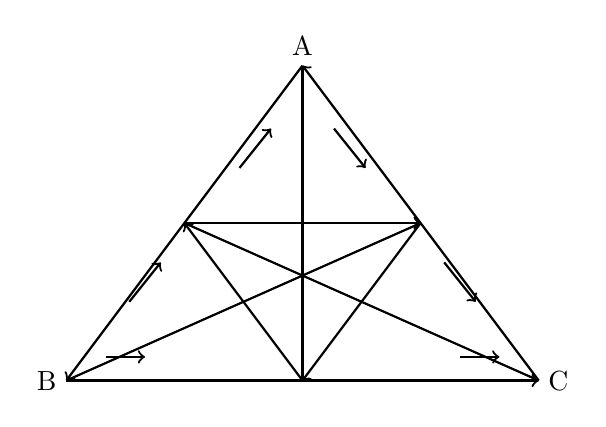
\begin{tikzpicture}
    \coordinate (A) at (0,4);
    \coordinate (B) at (-3,0);
    \coordinate (C) at (3,0);
    
    \coordinate (AB) at (-1.5,2);
    \coordinate (AC) at (1.5,2);
    \coordinate (BC) at (0,0);
    
    \coordinate (M) at (0,2);
    \coordinate (N) at (-1.5,1);
    \coordinate (O) at (1.5,1);
    
    \draw[thick, ->] (B) -- (C);
    \draw[thick, ->] (C) -- (A);
    \draw[thick, ->] (A) -- (B);
    
    \draw[thick, ->] (AB) -- (AC);
    \draw[thick, ->] (AC) -- (BC);
    \draw[thick, ->] (BC) -- (AB);
    
    \draw[thick] (A) -- (BC);
    \draw[thick] (B) -- (AC);
    \draw[thick] (C) -- (AB);
    
    \draw[thick,->] (-2.2,1) -- (-1.8,1.5);
    \draw[thick,->] (-0.8,2.7) -- (-0.4,3.2);
    \draw[thick,->] (1.8,1.5) -- (2.2,1);
    \draw[thick,->] (0.4,3.2) -- (0.8,2.7);
    \draw[thick,->] (-2.5,0.3) -- (-2.0,0.3);
    \draw[thick,->] (2.0,0.3) -- (2.5,0.3);

    \node[above] at (A) {A};
    \node[left] at (B) {B};
    \node[right] at (C) {C};
\end{tikzpicture}
\]
Let us consider the first original triangle $T^{(0)}$ with a positive orientation. Let $d^{(0)}$ and $p^{(0)}$ denote diameter and perimeter of $T^{(0)}$, respectively.
\\
\\
Now, bisecting the sides of triangle $T^{(0)}$, which yields four triangles, say $T^{(0)}_1$, $T^{(0)}_2$, $T^{(0)}_3$, $T^{(0)}_4$
Hence,
\[
\int_{T^{(0)}}f(z)dz=\sum_{j=1}^{4}\int_{T^{(1)}_j}f(z)dz
\]
By canceling the integration over the sides with opposite direction, we get
\[
\Big|\int_{T^{(1)}}f(z)dz\Big|\geq\Big|\int_{T^{(1)}_j}f(z)dz\Big|
\]
\[
\Rightarrow \Big|\int_{T^{(0)}}f(z)dz\Big|\leq4\Big|\int_{T^{(1)}}f(z)dz\Big|
\]
where $T^{(1)}$ is one among the four triangles with $d^{(1)}=\frac{1}{2}d^{(0)}$ and $p^{(1)}=\frac{1}{2}p^{(0)}$, where $d^{(1)}$ and $p^{(1)}$ denote the diameter and perimeter of triangle $T^{(1)}$, respectively.
\\
\\
Again, repeating the same process $n$-times, we obtain
\[
\Big|\int_{T^{(0)}}f(z)dz\Big|\leq4^n\Big|\int_{T^{(n)}}f(z)dz\Big|
\]
with $d^{(n)}=\frac{1}{2^n}d^{(0)}$ and $p^{(n)}=\frac{1}{2^n}p^{(0)}$, where $d^{(n)}$ and $p^{(n)}$ are diameter and perimeter of triangle $T^{(n)}$ respectively.
\\
\\
Since $f$ is holomorphic on $\Omega$, so it is holomorphic at $z_0\in \Omega$ and $f(z)=f(z_0)+f'(z_0)(z-z_0)+\psi(z)(z-z_0)$, where $\psi(z)\to 0$ as $z\to z_0$.
\\
\\
As $f(z_0)$ and $f'(z_0)$ are constants, the first two terms have primitives, thus, 
\[
\int_{T^{(n)}}[f(z_0)+f'(z_0)(z-z_0)]dz=0
\]
Thus,
\[
\int_{T^{(n)}}f(z)dz=\int_{T^{(n)}}\psi(z)(z-z_0)dz
\]
Now, $z_0$ belongs to the closure of solid triangle $\Delta^n$, and $z$ belongs to the boundary of $T^{(n)}$. Thus,
\[
|z-z_0|<d^{(n)}
\]
\[
\Big|\int_{T^{(n)}}f(z)dz\Big| \leq\epsilon_nd^{(n)}p^{(n)}
\]
where $\epsilon_n=Sup_{z\in T^{(n)}}|\psi(z)|\to 0$ as $n\to \infty$.
\[
\Rightarrow \Big|\int_{T^{(n)}}f(z)dz\Big| \leq \frac{\epsilon_nd^{(n)}p^{(n)}}{4^n}
\]
\[
\Rightarrow \Big|\int_{T^{(0)}}f(z)dz\Big|\leq4^n\Big|\int_{T^{(n)}}f(z)dz\Big|\leq\epsilon_nd^{(0)}p^{(0)}
\]
For $n\to \infty$, $\epsilon_n\to 0$. Therefore,
\[
\boxed{\int_{T}f(z)dz=0.}
\]
\qed
\\
\\
(b). If $f$ is holomorphic in an open set $\Omega$ that contains a rectangle $R$ and its interior then
\[
\int_{R}f(z)dz=0.
\]
\subsection{Local Existence of Primitives}
\textbf{Theorem.}
A holomorphic function in an open disc has a primitive in that disc.
\subsection{Cauchy's Integral in a Simply Connected Domain}
\textbf{Theorem.} If $f$ is holomorphic on a simply connected domain, then for every closed contour $C$,
\[
\int_{C}f(z)dz=0.
\]
\underline{Proof} Let $f(z)=u(x,y)+iv(x,y)$ be analytic on the domain $D$ where $z=x+iy$. Then,
\[
\int_{C}f(z)dz=\int_{C}(u+iv)(dx+idy)\\
\]
\[
=\int_{C}(udx+iudy+ivdx+i^2vdy)
\]
\[
=\int_{C}(udx-vdy)+i\int_{C}(vdx+udy)
\]
By \textbf{Green's Theorem},
\[
\int_{C}(Pdx+Qdy)=\iint_{R}(\frac{\partial Q}{\partial x}-\frac{\partial P}{\partial y})dxdy
\]
where $R$ is the region enclosed by $C$.
\[
\therefore \int_{C}(udx-vdy)=\iint_{R}(\frac{-\partial v}{\partial x}-\frac{\partial u}{\partial y})dxdy
\]
and
\[
\int_{C}(vdx+udy)=\iint_{R}(\frac{\partial u}{\partial x}-\frac{\partial v}{\partial y})dxdy
\]
Since $f$ is analytic, it satisfies the $C-R$ equations,
\[
\frac{\partial u}{\partial x}=\frac{\partial v}{\partial y}, \frac{\partial u}{\partial y}=\frac{-\partial v}{\partial x}
\]
\[
\therefore \int_{C}(udx-vdy)=\iint_{R}(\frac{\partial u}{\partial x}-\frac{\partial u}{\partial y})dxdy=0
\]
and
\[
\int_{C}(vdx+udy)=\iint_{R}(\frac{\partial v}{\partial x}-\frac{\partial v}{\partial y})dxdy=0
\]
Hence,
\[
\boxed{\int_{C}f(z)dz=0}
\]
\qed
\subsection{Cauchy's Integral Formula}
\textbf{Theorem.} If $f$ is an analytic function inside and on a closed contour $C$ and if $z_0$ be any point inside $C$ then
\[
\int_{C}\frac{f(z)}{z-z_0}dz=2\pi if(z_0)
\]
The integration being taken in counter clockwise.
\\
\\
\underline{Proof} Given that $f$ is analytic inside and on a simple closed contour $C$ and $z_0$ is any point inside $C$. Consider a disk $C_1$ centered at $z_0$ with radius $r$.
\[
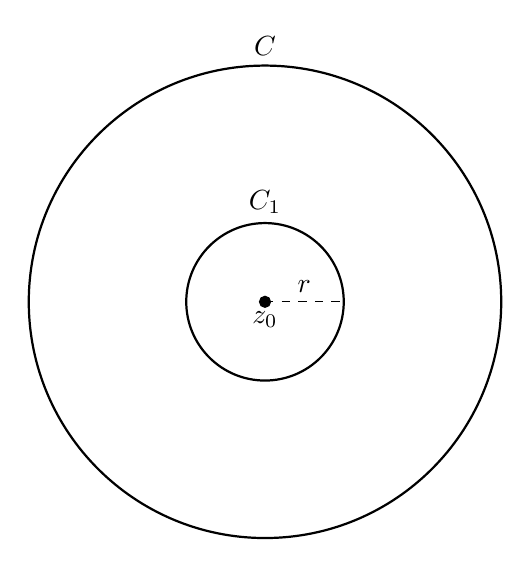
\begin{tikzpicture}
    \draw[thick] (0,0) circle (3cm);
    \node[above] at (0,3) {$C$};
    
    \draw[thick] (0,0) circle (1cm);
    \node[above] at (0,1) {$C_1$};
    
    \filldraw[black] (0,0) circle (2pt) node[below] {$z_0$};
    
    \draw[dashed] (0,0) -- (1,0) node[midway, above] {$r$};
    
\end{tikzpicture}
\]
So, 
\[
|z-z_0|=r
\]
\[
z-z_0=re^{i\theta}
\]
\[
\Rightarrow dz=rie^{i\theta}d\theta
\]
Clearly, $\frac{f(z)}{z-z_0}$ is analytic in $C-C_1$, So
\[
\int_{C-C_1}\frac{f(z)}{z-z_0}dz=0
\]
\[
\Rightarrow \int_{C}\frac{f(z)}{z-z_0}dz=\int_{C_1}\frac{f(z)}{z-z_0}dz
\]
\[
\Rightarrow \int_{C}\frac{f(z)}{z-z_0}dz=\int_{C_1}\frac{f(z_0+re^{i\theta})}{re^{i\theta}}rie^{i\theta}d\theta
\]
\[
\Rightarrow \int_{C}\frac{f(z)}{z-z_0}dz = i\int_{C_1}f(z_0+re^{i\theta})d\theta
\]
When $r\to 0$, then $f(z)\to f(z_0)$.
\[
\therefore \int_{C}\frac{f(z)}{z-z_0}=i\int_{C_1}f(z_0)d\theta
\]
\[
=if(z_0)\int_{0}^{2\pi}d\theta
\]
\[
=2\pi if(z_0)
\]
Therefore \[
\boxed{\displaystyle\int_{C}\frac{f(z)}{z-z_0}dz=2\pi if(z_0)}
\]
\qed
\subsection{Problems on Cauchy's Integral Formula}
1. Evaluate $\displaystyle\int_{C}\frac{dz}{z-3i}$ where $C$ is the circle $|z|=\pi$ counter clockwise.
\\
\\
\textbf{Solution.} The singularities of $F(z)=\frac{1}{z-3i}$ is given by
\[
z-3i=0
\]
\[
\Rightarrow z=3i
\]
which lies inside the circle $|z|=\pi=3.141$ and here $f(z)=1$.
\\
\\
Using Cauchy's Integral Formula,
\[
\displaystyle\int_{C}\frac{dz}{z-3i}=2\pi if(3i)
\]
\[
=2\pi i(1)
\]
\[
=2\pi i
\] 
\qed
\\
2. Evaluate $\displaystyle\int_{C}\frac{z}{(9-z^2)(z+1)}dz$ where $C$ is the circle $|z|=2$ counter clockwise.
\\
\\
\textbf{Solution.} The singularities of $F(z)=\frac{z}{(9-z^2)(z+1)}$ are given by
\[
(9-z^2)(z+1)=0
\]
\[
\Rightarrow 9-z^2=0, z+1=0
\]
\[
\Rightarrow z=\pm3,z=-1
\]
But the pole $z=\pm3$ lies outside the circle $|z|=2$, so
\[
\int_{C}\frac{z}{(9-z^2)(z+1)}dz=\int_{C}\frac{\frac{z}{9-z^2}}{z-(-1)}dz
\]
Here $f(z)=\frac{z}{9-z^2}$
\\
\[
\int_{C}\frac{z}{(9-z^2)(z+1)}dz=2\pi\ if(-1)
\]
\[
=2\pi i(\frac{-1}{9-1})
\]
\[
=2\pi i(\frac{-1}{8})
\]
\[
=\frac{-1}{4}\pi i
\]
\qed
\\
3. Evaluate $\displaystyle\int_{C}\frac{3z-1}{z^3-z}dz$ where $C$ is the circle
\[
a. |z|=\frac{1}{2}
\]
\[
b. |z|=2
\]
\\
\\
\textbf{Solution} The singularities of $F(z)=\frac{3z-1}{z^3-z}$ are given by
\[
z^3-z=0
\]
\[
\Rightarrow z(z^2-1)=0
\]
\[
\Rightarrow z=0, z^2-1=0
\]
\[
\Rightarrow z=0, z=\pm1
\]
a. For the circle $|z|=\frac{1}{2}$, the poles $z=\pm1$ do not lie inside. So,
\[
\int_{C}\frac{3z-1}{z^3-z}dz=\int_{C}\frac{\frac{3z-1}{z^2-1}}{z}dz
\]
Here $f(z)=\frac{3z-1}{z^2-1}$.
\\
\\
\[
\Rightarrow \int_{C}\frac{3z-1}{z^3-z}dz=2\pi if(0)
\]
\[
=2\pi i\Big(\frac{-1}{-1}\Big)
\]
\[
2\pi i
\]
\qed
\\
\\
b. For the circle $|z|=2$, all the singularities lie inside. So,
\[
F(z)=\frac{3z-1}{z(z-1)(z+1)}=\frac{A}{z}+\frac{B}{z-1}+\frac{C}{z+1}
\]
\[
\Rightarrow \frac{3z-1}{z(z-1)(z+1)}=\frac{A(z^2-1)+Bz(z+1)+Cz(z-1)}{z(z-1)(z+1)}
\]
\[
\Rightarrow 3z-1=Az^2-A+Bz^2+Bz+Cz^2-Cz
\]
\[
\Rightarrow 3z-1=(A+B+C)z^2+(B-C)z-A
\]
By comparing the coefficients of the powers of $z$,
\[
\boxed{A=1}
\]
\[
A+B+C=0 \Rightarrow B+C=-1
\]
\[
B-C=3
\]
\[
\Rightarrow 2B=2\Rightarrow \boxed{B=1}
\]
\[
\Rightarrow 1-C=3
\]
\[
\Rightarrow -C=2\Rightarrow \boxed{C=-2}
\]
Therefore,
\[
\int_{C}\frac{3z-1}{z^3-z}dz=\int_{C}\frac{dz}{z}+\int_{C}\frac{dz}{z-1}+\int_{C}\frac{-2dz}{z-(-1)}
\]
\[
=2\pi if(0)+2\pi if(1)+(-2)2\pi if(-1)
\]
\[
=2\pi i(1)+2\pi i(1)-4\pi i(1)=0
\]
\qed
\newpage
4. Evaluate $\displaystyle\int_{C}\frac{z+4}{z^2+2z+5}dz$ where $C$ is the circle $|z+1-i|=2$.
\\
\\
\textbf{Solution} The given circle is,
\[
|z+1-i|=2
\]
\[
\Rightarrow|z-(i-1)|=2
\]
\\
The singularities of $F(z)=\frac{z+4}{z^2+2z+5}$ are given by
\[
z^2+2z+5=0
\]
\[
\Rightarrow z=\frac{-2\pm\sqrt{2^2-4.1.5}}{2.1}
\]
\[
\Rightarrow z=\frac{-2\pm\sqrt{-16}}{2}
\]
\[
\Rightarrow z=\frac{-2\pm4i}{2}
\]
\[
\Rightarrow z=-1\pm 2i \Rightarrow z=-1+2i, -1-2i
\]
Now,
\[
|(-1+2i)-(i-1)|
\]
\[
=|-1+2i-i+1|
\]
\[
=|i|=1<2
\]
So, $-1+2i$ lies in the circle $|z+1-i|=2$.
\[
|(-1-2i)-(i-1)|
\]
\[
|-1-2i-i+1|=|-3i|=3>2
\]
So, $-1-2i$ lies outside the circle. Then,
\[
\int_{C}\frac{z+4}{z^2+2z+5}dz=\int_{C}\frac{\frac{z+4}{z+1+2i}}{z-(-1+2i)}dz
\]
Here $f(z)=\frac{z+4}{z+1+2i}$
\[
\Rightarrow \int_{C}\frac{z+4}{z^2+2z+5}dz=2\pi if(-1+2i)
\]
\[
=2\pi i\Big(\frac{-1+2i+4}{-1+2i+1+2i}\Big)
\]
\[
=2\pi i\Big(\frac{3+2i}{4i}\Big)=\frac{\pi}{2}(3+2i)
\]
\qed
\newpage
5. Evaluate $\displaystyle\int_{C}\frac{zdz}{z^4-1}$ where $C$ is the circle $|z-2|=2$.
\\
\\
\textbf{Solution} The singularities of $F(z)=\frac{z}{z^4-1}$ are given by
\[
z^4-1=0
\]
\[
\Rightarrow (z^2+1)(z^2-1)=0
\]
\[
\Rightarrow z^2+1=0, z^2-1=0
\]
\[
\Rightarrow z=\pm i,z=\pm 1
\]
For $z=\pm i$, $|\pm i-2|=\sqrt{5}>2$, so $z=\pm i$ lie outside the circle.
\\
For $z=1$, $|1-2|=1<2$, so it lies inside the circle, for $z=-1$, it lies outside the circle. Then,
\[
\int_{C}\frac{z}{z^4-1}dz=\int_{C}\frac{\frac{z}{(z^2+1)(z+1)}}{z-1}dz
\]
Here $f(z)=\frac{z}{(z^2+1)(z+1)}$,
\[
\int_{C}\frac{z}{z^4-1}dz=2\pi if(1)
\]
\[
=2\pi i\frac{1}{(1+1)(1+1)}
\]
\[
=2\pi i\frac{1}{4}
\]
\[
=\frac{\pi}{2}i
\]
\qed
\end{document}